\documentclass[11pt]{article}

\usepackage[margin=1in]{geometry}
\usepackage[utf8]{inputenc}
\usepackage[T1]{fontenc}
\usepackage{times}
\usepackage{amsmath,amssymb}
\usepackage{graphicx}
\usepackage{booktabs}
\usepackage{hyperref}
\usepackage{xcolor}
\usepackage{enumitem}
\usepackage{subcaption}
\usepackage{microtype}
\usepackage{authblk}
\usepackage{titling}

\setlength{\droptitle}{-1cm}
\pretitle{\begin{center}\Large\bfseries}
\posttitle{\end{center}\vspace{0.3cm}}

\hypersetup{
  colorlinks=true,
  linkcolor=black,
  citecolor=blue!50!black,
  urlcolor=blue!50!black
}

\title{Compute-Retrieve Axis: Detecting Reasoning Mode from Transformer Hidden States}

\author{
  Sam Ramdan\\
  Independent Researcher\\
  \texttt{sr4729820@gmail.com}\\[4pt]
  {\small Code and data: \url{https://github.com/Somebodyhere101/compute-retrieve}}
}

\begin{document}

\maketitle

\begin{abstract}
When a language model gets a question wrong, existing probes can detect the error but cannot say whether the model failed to recall a fact or failed to carry out a computation. We show that a single linear direction in transformer hidden states, the compute-retrieve (CR) axis, separates these two failure modes. Within individual subjects (physics, mathematics, geography), the axis distinguishes recall questions from computation questions at AUC~=~0.996--1.000. Among wrong answers on MMLU, it classifies reasoning-subject errors versus factual-subject errors at AUC~=~0.878--0.951 across three models. The axis generalizes across twelve models from five architecture families (70M--30B parameters) including LLaMA, and is nearly orthogonal to correctness (AUC~=~0.27). Detection requires one dot product on a single layer's hidden state, with no training or model modification.
\end{abstract}

\section{Introduction}

Large language models produce correct outputs through different internal processes. Answering ``What is the capital of France?'' retrieves a memorized fact; answering ``What is 347~+~289?'' requires computing a new result. When these operations fail, the causes differ: retrieval errors reflect incorrect associations stored during training, while computation errors reflect flawed reasoning applied to the input.

Truthfulness probes \citep{li2023iti, burns2022discovering, marks2024geometry} cannot make this distinction. They find directions in hidden state space that separate true from false, but both ``Paris'' (correct retrieval) and ``636'' (correct computation) register as truthful. Both retrieval errors and reasoning errors register as false. The probe collapses two dimensions of variation into one, discarding the mechanistic distinction.

We identify this missing axis. In transformer hidden state space, a single linear direction, the compute-retrieve (CR) axis, separates computation from retrieval across every model we tested. Following the representation engineering framework of \citet{zou2023representation}, the axis is the normalized mean difference between hidden states on computation-heavy and retrieval-heavy prompts.

Correctness is orthogonal. Table~\ref{tab:framework} shows the result of crossing mode with correctness: truthfulness probes measure the rows, the CR axis measures the columns.

\begin{table}[ht]
\caption{Crossing mode with correctness produces four categories. Truthfulness probes measure rows; the CR axis measures columns.}
\vspace{4pt}
\centering
\renewcommand{\arraystretch}{1.5}
\begin{tabular}{l cc}
\toprule
 & \textbf{Retrieve} & \textbf{Compute} \\
\midrule
\textbf{Correct} & Recall & Reasoning \\
\textbf{Wrong}   & Retrieval error & Reasoning error \\
\bottomrule
\end{tabular}
\renewcommand{\arraystretch}{1.0}
\label{tab:framework}
\end{table}

We validate the axis on twelve models from five architecture families (including LLaMA), on 320 questions from four standard benchmarks, and through eleven controls designed to rule out confounds. Within bare arithmetic, it tracks difficulty monotonically ($r$~=~0.951), rising smoothly from ``What is 1+1?'' to ``What is 1847$\times$3?'' with the same prompt format throughout. The gradient replicates on Qwen~2.5 at $r$~=~0.74--0.84.

However, the axis direction depends on calibration prompts. Axes calibrated on arithmetic versus logic prompts are nearly orthogonal (cosine~=~0.08), though each works on its own domain at AUC~$\geq$~0.85. Separation is consistent across domains, but the specific direction is calibration-dependent. The difficulty gradient also only works on bare arithmetic, not word problems; GSM8K difficulty and projection are uncorrelated. The axis measures computational effort on simple tasks, not general problem difficulty.

\paragraph{Contributions.} (1) We demonstrate that the CR axis classifies failure types on MMLU: among wrong answers in the same multiple-choice format, it distinguishes reasoning-subject errors from factual-subject errors at AUC~=~0.878--0.951, and within-subject controls confirm this reflects computational demand, not subject identity (Section~\ref{sec:analysis}). (2) We validate the axis across architectures, benchmarks, and eleven controls for format, length, domain, and within-subject confounds (Section~\ref{sec:results}). (3) We report five failed intervention attempts that constrain what can be done with the axis (Section~\ref{sec:analysis}).

\section{Related Work}

Several lines of work probe transformer hidden states for structured information. Truthfulness probes \citep{li2023iti, burns2022discovering, marks2024geometry, azaria2023internal} find linear directions that separate true from false statements, and \citet{kadavath2022language} show models can self-evaluate correctness. These all operate along the correctness axis of the 2$\times$2 (Table~\ref{tab:framework}). The CR axis operates along the orthogonal mode axis, capturing \emph{how} the model produced its output rather than \emph{whether} the output is correct.

Our method, mean difference on contrast pairs, is representation engineering \citep{zou2023representation}, the same technique used for honesty and harmlessness directions. The contribution is the target, not the method: RepE concepts are properties of output behavior, while computational mode is a property of internal processing. The same wrong answer can arise from either mode, which is why truthfulness probes alone cannot make the distinction that failure classification requires. \citet{todd2024function} find related linear directions for in-context task types but do not test failure classification or cross-architecture transfer. Our work extends the RepE framework to process-level rather than output-level concepts, and demonstrates that mode and correctness capture genuinely different information (AUC~=~0.27 on correct-vs-wrong).

At the circuit level, \citet{geva2023dissecting} trace how transformers recall factual associations through specific attention heads and MLP layers; the retrieve-mode signal we detect likely reflects the same circuitry measured globally. Circuit-level methods \citep{nanda2023grokking, conmy2023automated, elhage2022superposition} offer more mechanistic detail but require substantially more analysis per model. Gate map diffing, which we use as an auxiliary tool, sits between these approaches: it identifies correlated patterns quickly but not causal mechanisms, as our ablation results confirm (Section~\ref{sec:analysis}). Finally, hidden-state probes for hallucination detection are increasingly common, but they predict wrong outputs regardless of cause. The CR axis splits what is commonly called ``hallucination'' into retrieval errors and reasoning errors. Whether this distinction matters for mitigation remains an open empirical question.

\section{Method}\label{sec:method}

\subsection{Axis Computation}

Given a model with $L$ transformer layers, we extract the hidden state $\mathbf{h}_l$ at layer $l$, last token position, via a hook during a standard forward pass. No weights are modified.

We collect hidden states for two sets of calibration prompts: $\mathcal{C} = \{c_1, \dots, c_n\}$ requiring active computation and $\mathcal{R} = \{r_1, \dots, r_m\}$ requiring memory retrieval. From these, we define the CR axis as:
\begin{equation}
\hat{\mathbf{a}} = \frac{\bar{\mathbf{h}}_{\mathcal{C}} - \bar{\mathbf{h}}_{\mathcal{R}}}{\|\bar{\mathbf{h}}_{\mathcal{C}} - \bar{\mathbf{h}}_{\mathcal{R}}\|}
\label{eq:axis}
\end{equation}
where $\bar{\mathbf{h}}_{\mathcal{C}} = \frac{1}{n}\sum_i \mathbf{h}_l(c_i)$ and likewise for $\bar{\mathbf{h}}_{\mathcal{R}}$. For a new prompt $p$, the CR projection is $\text{proj}(p) = \mathbf{h}_l(p) \cdot \hat{\mathbf{a}}$. Positive values indicate compute mode; negative values indicate retrieve mode.

\subsection{Layer Selection}

We test candidate layers at approximately 25\%, 50\%, 75\% depth and near the final layer, selecting the one with the highest AUC on the calibration data. To verify this does not overfit to calibration data, we run 5-fold stratified cross-validation on Gemma~4~E2B: each fold selects the best layer on training data and evaluates on held-out calibration prompts. All five folds select the same layer (L17), with mean test AUC~=~0.994~$\pm$~0.011. Across all tested architectures, the best layer falls between 25\% and 75\% depth.

\subsection{Calibration Requirements}

We use 30 GSM8K questions \citep{cobbe2021gsm8k} as compute calibration and 30 MMLU questions \citep{hendrycks2021mmlu} as retrieve calibration. Table~\ref{tab:robustness_inline} shows that 15 prompts per class suffice for a stable axis.

\begin{table}[h]
\caption{Fifteen prompts per class suffice for a stable axis (cos $>$ 0.93 to the full-data direction, 20 random trials per size).}
\label{tab:robustness_inline}
\vspace{4pt}
\centering
\small
\begin{tabular}{@{}lc@{}}
\toprule
Prompts per class & Cosine to full axis \\
\midrule
5 & 0.81 $\pm$ 0.09 \\
10 & 0.91 $\pm$ 0.04 \\
15 & 0.94 $\pm$ 0.02 \\
30 & 0.98 $\pm$ 0.007 \\
\bottomrule
\end{tabular}
\end{table}

\subsection{Cost}

Calibration takes 1.6\,s for 60 prompts on a single GPU (RTX~5090). Detection takes 42\,ms per prompt: one forward pass plus one dot product. Storage is one vector (6\,KB). The method requires no training, no learned parameters, and no model modification.

\section{Experiments}\label{sec:results}

\subsection{Multi-Architecture Validation}

We tested twelve models from five architecture families: Pythia \citep{biderman2023pythia} (70M, 160M, 410M, 1B), Qwen~2.5 (0.5B, 1.5B, 3B, 7B), Gemma~4 (E2B, E4B), Qwen3-30B-A3B (mixture-of-experts, 30B total, 3B active), and LLaMA~3.2-1B \citep{grattafiori2024llama}. Table~\ref{tab:models} summarizes the results.

\begin{table}[t]
\caption{The CR axis achieves AUC $\geq$ 0.988 across twelve models from five architecture families spanning 70M to 30B parameters. $d$: Cohen's $d$. Grad $r$: difficulty--projection correlation. $^\ddagger$Validated via controls only ($N$~=~10, not a gradient).}
\label{tab:models}
\vspace{4pt}
\centering
\small
\begin{tabular}{@{}llcccc@{}}
\toprule
Model & Params & Layer & AUC & $d$ & Grad $r$ \\
\midrule
Pythia-70M & 70M & L1 & 0.988 & 3.13 & 0.27 \\
Pythia-160M & 160M & L3 & 1.000 & 2.95 & 0.62 \\
Pythia-410M & 410M & L6 & 1.000 & 2.82 & 0.51 \\
Pythia-1B & 1B & L4 & 1.000 & 2.94 & 0.28 \\
\midrule
Qwen2.5-0.5B & 0.5B & L12 & 1.000 & 3.95 & 0.84 \\
Qwen2.5-1.5B & 1.5B & L21 & 1.000 & 3.52 & 0.77 \\
Qwen2.5-3B & 3B & L9 & 1.000 & 3.07 & 0.74 \\
Qwen2.5-7B & 7B & L21 & 1.000 & 3.18 & 0.77 \\
\midrule
Gemma-4-E2B & 2.3B & L26 & 1.000 & 3.10 & 0.94 \\
Gemma-4-E4B & 8B & L40 & 0.994 & 3.00 & 0.68 \\
\midrule
Qwen3-30B-A3B & 30B & L36 & 0.997 & 3.50 & 0.85 \\
\midrule
LLaMA-3.2-1B & 1.2B & L12 & 1.000 & $^\ddagger$ & $^\ddagger$ \\
\bottomrule
\end{tabular}
\end{table}

Separation reaches AUC~$\geq$~0.988 in every model (Figure~\ref{fig:multimodel}), including the Pythia base models (no instruction tuning) and LLaMA~3.2-1B. Gradient correlation is strongest on instruction-tuned models ($r$~=~0.74--0.94) and weakest on base models ($r$~=~0.27--0.62). The format control confirms this pattern: matched-format pairs separate at 35/35 (Gemma), 20/20 (Qwen~0.5B), and 20/20 (LLaMA~1B) on instruction-tuned models, but only 3/20 on Pythia-410M (base). Mode separation on the calibration data (AUC~$\geq$~0.988) holds even on base models, but finer-grained distinctions require instruction tuning.

\begin{figure}[t]
\centering
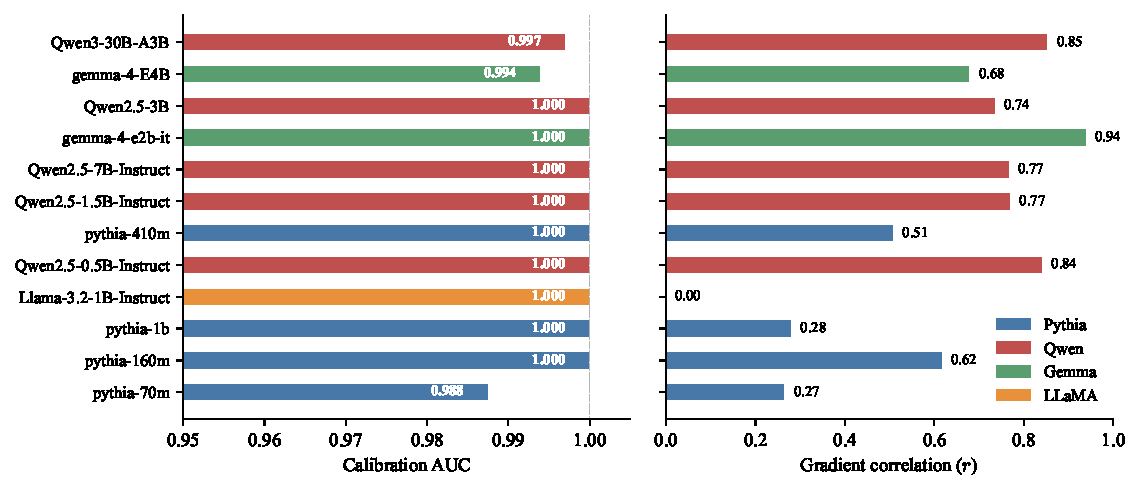
\includegraphics[width=0.85\textwidth]{figures/fig7_multimodel.pdf}
\caption{All twelve models achieve AUC $\geq$ 0.988 (left). Gradient correlation is stronger on instruction-tuned models (right).}
\label{fig:multimodel}
\end{figure}

\subsection{Standard Benchmarks}

The axis was calibrated on 30 GSM8K questions and 30 MMLU questions, then tested on held-out data. Table~\ref{tab:benchmarks} shows the results.

\begin{table}[t]
\caption{The axis transfers to held-out and unseen benchmarks without recalibration, achieving AUC = 1.000 on cross-benchmark data and 0.927 within MMLU subjects.}
\label{tab:benchmarks}
\vspace{4pt}
\centering
\small
\begin{tabular}{@{}lrcc@{}}
\toprule
Test & $N$ & AUC & $d$ \\
\midrule
Calibration (GSM8K + MMLU) & 60 & 1.000 & 4.00 \\
Held-out (GSM8K + MMLU) & 100 & 1.000 & 4.05 \\
Cross-benchmark (AQUA-RAT + OpenBookQA) & 60 & 1.000 & 7.80 \\
MMLU reasoning vs.\ factual subjects & 100 & 0.927 & 2.14 \\
\bottomrule
\end{tabular}
\end{table}

Held-out data consists of 50 GSM8K and 50 MMLU questions not used in calibration. Between-benchmark separation is perfect (AUC~=~1.000), though this is expected: the held-out data comes from the same distributions as calibration, and GSM8K and MMLU differ in surface features. The sharper test is within-benchmark: among MMLU questions alone, reasoning-heavy subjects (physics, mathematics) project higher than factual subjects (world religions, geography) at AUC~=~0.927 (Figure~\ref{fig:benchmarks}). The axis transfers across benchmarks without recalibration: calibrated on GSM8K and MMLU, it separates AQUA-RAT from OpenBookQA at AUC~=~1.000 with $d$~=~7.80.

Token length and CR projection are uncorrelated on benchmark data ($r$~=~$-$0.089).

\begin{figure}[t]
\centering
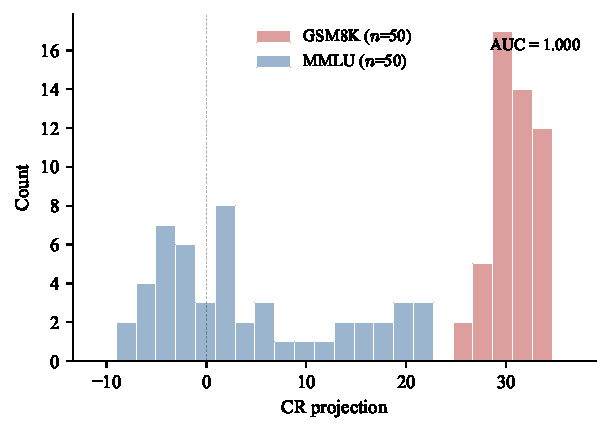
\includegraphics[width=0.65\textwidth]{figures/fig4_benchmarks.pdf}
\caption{Held-out GSM8K (red) vs.\ MMLU (blue) projections. AUC~=~1.000.}
\label{fig:benchmarks}
\end{figure}

\subsection{Controls}\label{sec:controls}

Table~\ref{tab:controls} summarizes the control experiments.

\begin{table}[t]
\caption{Eleven controls rule out format, length, subject identity, architecture, and calibration confounds. All on Gemma~4~E2B except cross-architecture rows.}
\label{tab:controls}
\vspace{4pt}
\centering
\small
\begin{tabular}{@{}llcl@{}}
\toprule
Control & $N$ & Result & Confound addressed \\
\midrule
Format-matched pairs & 35 & 35/35 separated & Prompt format \\
Within-arithmetic & 30 & AUC = 1.000, $d$ = 4.16 & Domain \\
Within-subject (3 subjects) & 90 & AUC = 0.996--1.000 & Subject identity \\
Reversed length & 30 & 30/30, $d$ = 8.48 & Token count \\
Benchmark length corr. & 100 & $r$ = $-$0.089 & Token count \\
Adversarial prompts & 50 & AUC = 0.998 [0.992, 1.000] & Surface features \\
Cross-arch (Qwen 0.5B) & 40 & 20/20 fmt, 20/20 len & Architecture \\
Cross-arch (LLaMA 1B) & 40 & 20/20 fmt, 20/20 len & Architecture \\
Cross-arch (Pythia 410M) & 40 & 3/20 fmt, 20/20 len & Base model \\
Robustness ($n$=15) & 20 trials & cos = 0.94 & Calibration instability \\
Cross-domain & 4 axes & cos = 0.08--0.70 & Direction universality \\
\bottomrule
\end{tabular}
\end{table}

\paragraph{Format control.} We constructed 35 prompt pairs with matched surface features (both use ``What is~\ldots?'') where one requires computation and one requires retrieval. All 35 separate correctly.

\paragraph{Within-arithmetic.} All prompts follow ``What is X op Y?''. Only the numbers differ. Trivial arithmetic ($1+1$, $2+2$) projects at $+$12.5 on average; hard arithmetic ($347+289$, $23\times19$) projects at $+$22.5. AUC~=~1.000, $d$~=~4.16.

\paragraph{Ruling out length.} We made compute prompts deliberately short (``47*38='', 6 tokens) and retrieve prompts deliberately long (``According to established historical records, the capital city of\ldots'', 19 tokens). If the axis measured length, short prompts would project lower. All 30 pairs separate correctly with $d$~=~8.48.

\paragraph{Calibration robustness.} At 15 prompts per class, the cosine to the full-data axis is 0.94 (Figure~\ref{fig:robustness}). At 30, it is 0.98.

\begin{figure}[t]
\centering
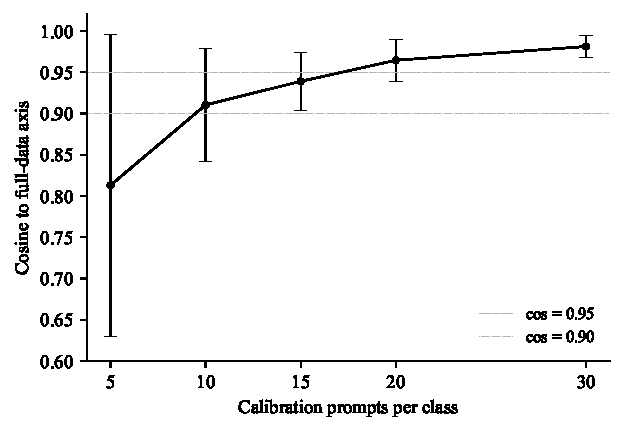
\includegraphics[width=0.55\textwidth]{figures/fig6_robustness.pdf}
\caption{The axis converges rapidly: 15 prompts per class yield cos $>$ 0.93 to the full-data axis (20 trials per size).}
\label{fig:robustness}
\end{figure}

\paragraph{Adversarial prompts.} The strongest confound test uses 50 prompts designed to mismatch surface features with computational mode. Math-looking retrieval prompts (``What is Avogadro's number?'', ``What is the atomic number of gold?'') require pure recall. Trivia-looking computation prompts (``If apples cost \$1.20 each and I buy 8, how much change from \$20?'') require active calculation despite their colloquial framing. The axis classifies them at AUC~=~0.998 (95\% CI [0.992, 1.000]) with $d$~=~5.27: math-looking retrieval projects at $+$7.6 on average, trivia-looking computation at $+$23.5. Surface features do not drive the separation. A limitation of this test is that the retrieval prompts are mostly short factoid lookups while the computation prompts are longer word problems, so prompt complexity remains a potential confound even though the reversed-length control argues against pure length effects.

\paragraph{Within-subject control.} A concern with the failure classification experiment (Section~\ref{sec:analysis}) is that the axis might track \emph{subject identity} rather than \emph{failure mode}. We constructed 15 recall and 15 computation questions within each of three subjects: physics, mathematics, and geography. For example, within physics: ``What is the SI unit of force?'' (recall) versus ``A 10\,kg box slides down a 30-degree frictionless incline. What is its acceleration?'' (computation). Within every subject, the axis distinguishes recall from computation: physics AUC~=~1.000 ($d$~=~4.36), mathematics AUC~=~0.996 ($d$~=~3.20), geography AUC~=~1.000 ($d$~=~6.88). The axis measures computational demand, not subject identity.

\paragraph{Cross-architecture replication.} The format and reversed-length controls replicate on other architectures. On Qwen~2.5~0.5B: 20/20 format and 20/20 reversed-length ($d$~=~8.5). On LLaMA~3.2-1B: 20/20 format and 20/20 reversed-length ($d$~=~12.4); within-subject physics AUC~=~0.990. On Pythia-410M (base model): 20/20 reversed-length ($d$~=~2.8), but only 3/20 format pairs. Base models without instruction tuning do not cleanly distinguish matched-format prompts by computational demand, consistent with the weaker gradient correlations for Pythia in Table~\ref{tab:models}. The length control holds across all architectures and all model families tested.

\paragraph{Baseline comparison.} On the adversarial test set, a logistic regression trained on calibration hidden states achieves AUC~=~0.984, slightly worse than our untrained mean-difference axis (0.998). PCA's first component achieves AUC~=~1.000, meaning compute/retrieve is the dominant axis of variation in the calibration hidden states; this depends on the calibration mix and would not necessarily hold on other prompt distributions. Random axes average AUC~=~0.67. The cosine between the logistic regression direction and the mean-difference direction is 0.74, indicating a broad cone of effective directions rather than a single precise vector. The mean-difference direction is the simplest of these and slightly outperforms the trained alternative on small calibration sets.

\paragraph{Cross-domain direction.} On Gemma~4~E2B, arithmetic and logic axes have cosine 0.08. On Qwen~7B, the same pair has cosine 0.40, and other pairs range from 0.36 to 0.70. The degree of cross-domain alignment is architecture-dependent. PCA on four domain-specific axes (arithmetic, logic, causal, sequence) from Qwen shows that one dimension captures 56\% of variance and two dimensions capture 80\%. The per-domain axes thus share a low-dimensional subspace of 2--3 dimensions rather than spanning the full hidden state space. The CR axis is a family of related directions, more tightly clustered on some architectures than others.

\subsection{Difficulty Gradient}\label{sec:gradient}

Within bare arithmetic, the CR axis tracks computational difficulty as a continuous quantity. Figure~\ref{fig:gradient} shows 24 prompts, all in the format ``What is X op Y?'', with an ordinal memorization score (1--10) based on the assumption that common facts (e.g., $1+1$, $7 \times 8$) appear far more often in training corpora than uncommon products (e.g., $47 \times 38$). This ranking is subjective but monotonic by construction.

\begin{figure}[t]
\centering
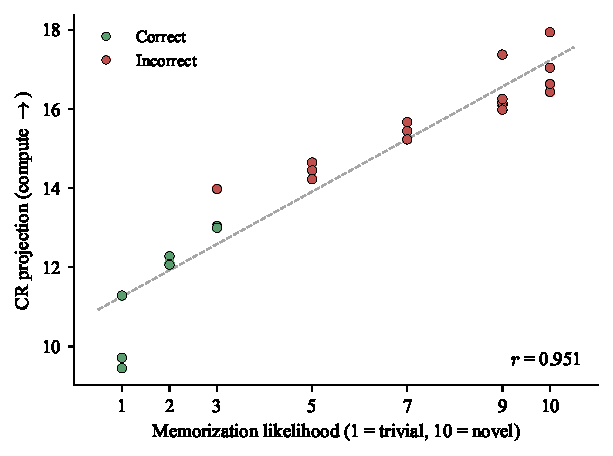
\includegraphics[width=0.65\textwidth]{figures/fig3_gradient.pdf}
\caption{CR projection vs.\ memorization likelihood for 24 arithmetic prompts ($r$~=~0.951, 95\% CI [0.890, 0.966]). Green: correct. Red: incorrect.}
\label{fig:gradient}
\end{figure}

On Gemma~4~E2B, $r$~=~0.951 (95\% CI [0.890, 0.966], 1000-sample bootstrap). After partialing out token length, $r$~=~0.711. Across Qwen~2.5, the same pattern holds ($r$~=~0.74--0.84), monotonic in every instruction-tuned model.

On base models (Pythia), the gradient is weaker ($r$~=~0.27--0.62) and not always monotonic. Mode separation still holds (calibration AUC $\geq$~0.988) but difficulty tracking is noisier.

However, the gradient does not extend to word problems. On GSM8K questions stratified by solution length, projection is flat: all GSM8K questions require active computation regardless of difficulty, so they all land in the compute region, as expected. The axis measures where a prompt falls on the compute-versus-retrieve spectrum. It does not measure how hard a problem is once the model is already in compute mode.

\section{Analysis}\label{sec:analysis}

\subsection{Classifying Failures on MMLU}

To test whether the 2$\times$2 framework applies to real model failures, we evaluated three models on 240 MMLU questions from 12 subjects: 6 reasoning-heavy (including physics, mathematics, chemistry) and 6 factual (including world religions, geography, anatomy, history). All questions are multiple choice with the same format. Among wrong answers only:

\begin{table}[h]
\caption{Among wrong answers on MMLU, the CR axis separates reasoning-subject errors from factual-subject errors at AUC 0.878--0.951, improving with model scale. R: reasoning. F: factual. $^\dagger$CI not computed.}
\label{tab:failure}
\vspace{4pt}
\centering
\small
\begin{tabular}{@{}lcccccc@{}}
\toprule
Model & Wrong (R) & Wrong (F) & Proj (R) & Proj (F) & AUC & 95\% CI \\
\midrule
Gemma-4-E2B & 116 & 117 & $+$10.1 & $-$2.2 & 0.878 & [0.830, 0.917] \\
Qwen2.5-7B & 119 & 119 & $+$14.2 & $-$10.5 & 0.885 & [0.846, 0.927] \\
Qwen3-30B & 119 & 120 & $+$1.5 & $-$7.9 & 0.951 & $^\dagger$ \\
\bottomrule
\end{tabular}
\end{table}

Wrong answers on reasoning subjects project higher (compute side) than wrong answers on factual subjects (retrieve side), with AUC~=~0.878--0.951, and separation improves with model scale. All wrong answers use the same multiple-choice format, so the axis is classifying failure type from the hidden state alone. A caveat: subject type is a proxy for failure mode, not a direct measure (a physics question can be answered from recall, and a geography question can require reasoning). The within-subject control (Section~\ref{sec:controls}) shows the axis distinguishes recall from computation within individual subjects on hand-crafted prompts, which helps but does not settle the question; expert annotation of individual MMLU questions by required mode would provide stronger evidence.

\subsection{Token-Level Dynamics}

Per-token CR projection during generation (Figure~\ref{fig:trajectories}) shows that compute tasks maintain positive projection throughout, while retrieve tasks start near zero and drift positive as the model transitions from stating the answer to explaining it. The first generated token provides the cleanest signal.

\begin{figure}[t]
\centering
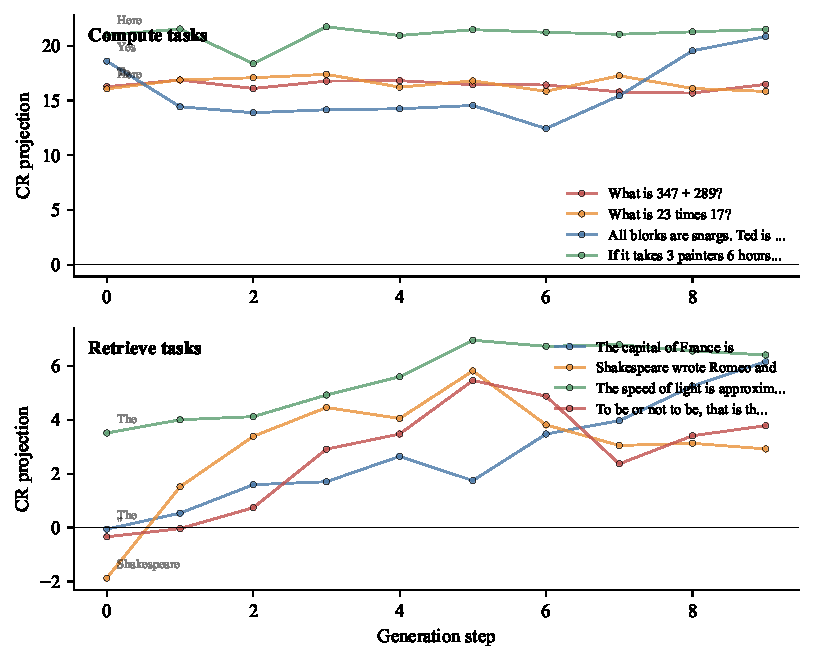
\includegraphics[width=0.85\textwidth]{figures/fig5_trajectories.pdf}
\caption{Compute tasks maintain positive projection throughout generation; retrieve tasks start near zero and drift positive during explanation.}
\label{fig:trajectories}
\end{figure}

\subsection{Failed Interventions}

We attempted five interventions using the CR axis to modify model behavior. None succeeded.

\begin{table}[t]
\caption{Five interventions attempted using the CR axis. All failed, each for a different structural reason.}
\label{tab:negatives}
\vspace{4pt}
\centering
\small
\begin{tabular}{@{}ll@{}}
\toprule
Intervention & Result \\
\midrule
Neuron ablation (L25) & cos = 1.000 (zero effect on output) \\
Self-reflection & cos = $-$0.44 (Gemma), $+$0.51 (Qwen) \\
Output layer modification & 0/11 answers corrected \\
Gate pattern transplant & Gibberish output \\
Hidden state injection & No effect on generation \\
\bottomrule
\end{tabular}
\end{table}

Two neurons at layer~25 in Gemma~4 flip their gate state for every reasoning prompt and never flip for non-reasoning prompts (0 false positives across 15 conditions). Yet ablating them changes nothing: output logit cosine is 1.0000 with or without them. They correlate perfectly with reasoning mode but play no causal role. Gate analysis identifies correlated neurons; ablation is needed to distinguish markers from mechanisms.

Self-reflection is architecture-dependent. On Gemma~4, asking ``what went wrong?'' produces a hidden state that points away from the correction (cosine~=~$-$0.44). On Qwen~7B, it points toward the correction (cosine~=~$+$0.51).

\section{Discussion}

The main limitation is the absence of causal evidence. We show that the CR axis \emph{correlates} with computational mode, but we have not demonstrated that intervening on this direction changes model behavior. \citet{marks2024geometry} provide causal evidence for truth representations via activation patching; an analogous experiment for the CR axis (shifting a model from retrieve mode to compute mode and observing changed outputs) would show whether the direction actually drives behavior, not just predicts it. The five failed interventions in Table~\ref{tab:negatives} underscore this gap.

The CR axis direction is calibration-dependent (arithmetic vs.\ logic cosine~=~0.08). The difficulty gradient holds on bare arithmetic but not word problems. Self-reflection anti-alignment does not replicate across architectures. We tested only English prompts. On Qwen~7B (8-bit, 200 MMLU questions, 140 correct), the CR axis predicts correctness at AUC~=~0.27, near chance, while a truthfulness probe distinguishes reasoning errors from retrieval errors at AUC~=~0.91, almost as well as the CR axis (0.94). The two directions have cosine $-$0.14, nearly orthogonal geometrically, but the truthfulness probe still carries mode information. The separation is incomplete: the CR axis is blind to correctness, but the truthfulness axis is not fully blind to mode.

\section{Conclusion}

A linear direction in transformer hidden states separates multi-step processing from single-step lookup across every architecture we tested. It correlates with but is not identical to a truthfulness direction: the CR axis is blind to correctness (AUC~=~0.27), and it slightly outperforms the truth probe on failure classification (0.94 vs 0.91). Whether this direction reflects a deep computational mode or a shallower proxy for prompt complexity remains open. The main practical result is that it reliably classifies failure types from a single hidden state, information that existing probes do not provide.

\section*{Acknowledgments}

This research made heavy use of Claude Opus 4.6 (Anthropic) via Claude Code for experimental design, implementation, data analysis, and writing. All AI-generated text and code was reviewed and verified by the author. Thanks to the Pythia, Qwen, Gemma, and LLaMA teams for open-sourcing their model weights.

\bibliographystyle{plainnat}
\bibliography{references}

\appendix
\section{Calibration Prompts}\label{app:prompts}

Compute calibration uses 30 prompts from GSM8K \citep{cobbe2021gsm8k}; retrieve calibration uses 30 from MMLU \citep{hendrycks2021mmlu}. Full prompt lists are in the repository at \texttt{data/calibration/}.

\section{Per-Model Gradient Details}\label{app:gradient}

\begin{table}[h]
\caption{Instruction-tuned models show monotonic difficulty gradients; base models do not. LLaMA omitted (gradient data collected separately).}
\vspace{4pt}
\centering
\small
\begin{tabular}{@{}lccccc@{}}
\toprule
Model & Low (1--3) & Mid (5--7) & High (9--10) & $r$ & Monotonic \\
\midrule
Pythia-70M & $+$4.0 & $+$3.9 & $+$4.3 & 0.27 & No \\
Pythia-160M & $+$8.3 & $+$8.5 & $+$8.6 & 0.62 & Yes \\
Pythia-410M & $+$11.0 & $+$11.7 & $+$11.6 & 0.51 & No \\
Pythia-1B & $+$19.6 & $+$19.7 & $+$20.3 & 0.28 & Yes \\
\midrule
Qwen2.5-0.5B & $+$3.3 & $+$4.0 & $+$4.1 & 0.84 & Yes \\
Qwen2.5-1.5B & $+$33.5 & $+$37.1 & $+$37.7 & 0.77 & Yes \\
Qwen2.5-3B & $+$31.6 & $+$33.6 & $+$33.6 & 0.74 & Yes \\
Qwen2.5-7B & $+$63.5 & $+$71.2 & $+$71.4 & 0.77 & Yes \\
\midrule
Gemma-4-E2B & $+$13.1 & $+$19.3 & $+$23.3 & 0.94 & Yes \\
Gemma-4-E4B & $+$26.7 & $+$32.2 & $+$31.9 & 0.68 & No \\
\midrule
Qwen3-30B-A3B & $-$1.3 & $+$2.1 & $+$2.7 & 0.85 & Yes \\
\bottomrule
\end{tabular}
\end{table}

\section{Bootstrap Confidence Intervals}\label{app:bootstrap}

1000-sample bootstrap on Gemma~4~E2B:

\begin{table}[h]
\caption{All key metrics remain significant under bootstrap resampling (1000 samples, Gemma 4 E2B).}
\vspace{4pt}
\centering
\small
\begin{tabular}{@{}lcc@{}}
\toprule
Metric & Point estimate & 95\% CI \\
\midrule
Calibration AUC & 1.000 & [1.000, 1.000] \\
Held-out AUC & 1.000 & [1.000, 1.000] \\
Adversarial AUC & 0.998 & [0.992, 1.000] \\
Failure AUC (Gemma E2B) & 0.878 & [0.830, 0.917] \\
Failure AUC (Qwen 7B) & 0.885 & [0.846, 0.927] \\
Cohen's $d$ & 4.11 & [3.53, 5.50] \\
Gradient $r$ & 0.951 & [0.890, 0.966] \\
\bottomrule
\end{tabular}
\end{table}

\section{Experimental Environment}\label{app:env}

All experiments were run on a single NVIDIA RTX~5090 (32\,GB) with CUDA~12.8, PyTorch~2.11.0, and Transformers~5.5.0. All generation uses greedy decoding (temperature~=~0). Results are deterministic: re-running produces axis cosine~=~1.000000 to the original.

\end{document}
